\section{Temperature Sensor}

\subsection{Introduction}
An RGB LED combines red, green, and blue light-emitting diodes
into a single package, allowing various colors to be displayed based
on the combination of the three. In this experiment, a common anode RGB
LED is used as a visual indicator to represent different temperature ranges
detected by a temperature sensor. The anode is connected to a positive
voltage, and individual colors are controlled by pulling their respective
cathodes low.

The analog signal from the temperature sensor is read by the
microcontroller and compared against predefined threshold values.
Depending on the temperature reading, the RGB LED lights up in blue,
green, or red to indicate cold, normal, or high temperature, respectively.
The logic is designed for common anode configuration, where writing LOW
to a pin turns that LED color on. This setup provides a simple and effective
way to visualize sensor data using colored light, demonstrating how analog 
inputs and digital outputs can be used together in real-time embedded systems.

\subsection{Procedure}
1. Gathered an STM32F103C6 Blue Pill board, common anode RGB LED, 
temperature sensor, three $220\Omega$ resistors, breadboard, and jumper wires.

2. Connected the common anode pin of the RGB LED to 3.3V.
Connected the red, green, and blue cathode pins to PB0, PB4, and PB3
respectively, each through a $220\Omega$ resistor.

3. Connected the temperature sensor's output to PB1 (analog input),
VCC to 3.3V, and GND to ground.

4. Verified all wiring for correctness and secure connections 
on the breadboard.

5. Uploaded the code via PlatformIO. The RGB LED lit up in different
colors (blue, green, or red) based on the temperature sensor's reading,
indicating low, normal, or high temperature.
\newpage
\subsection{Diagram}
\begin{figure}[htbp]
    \centering
    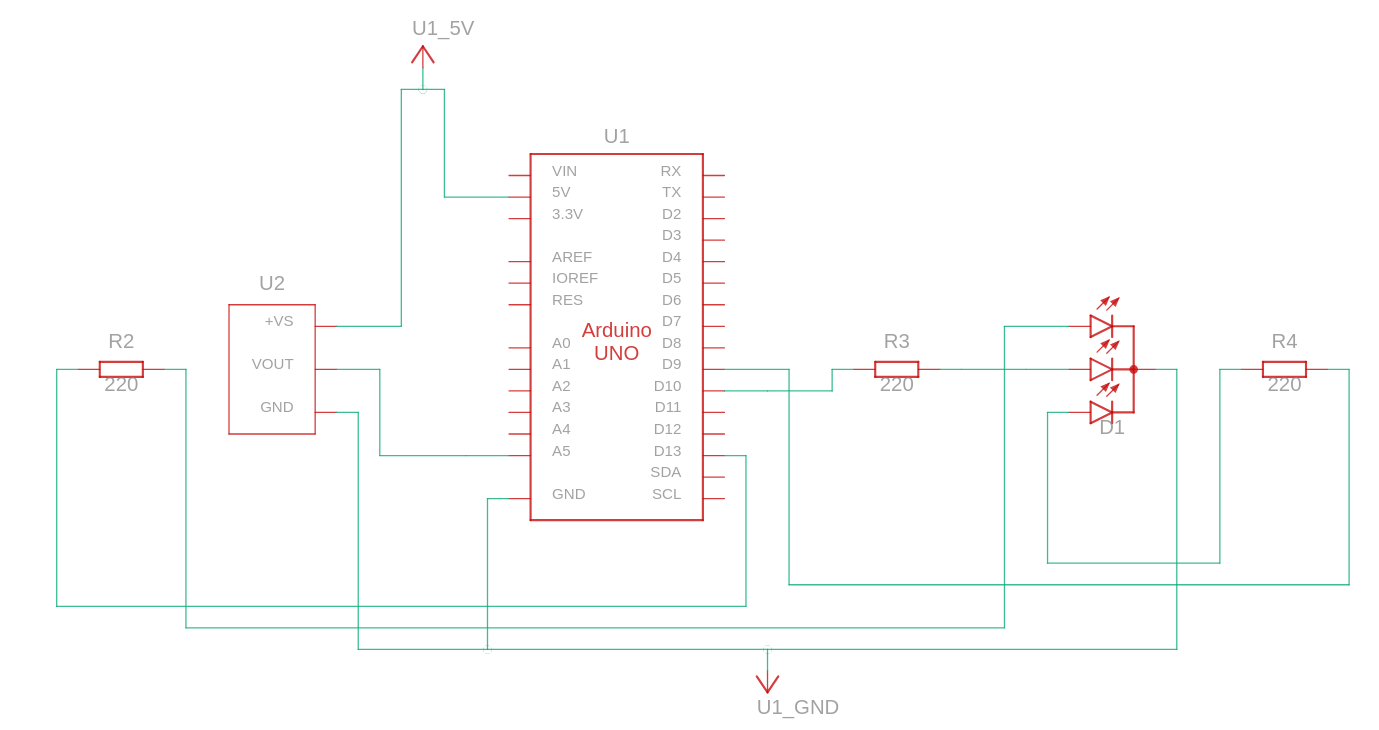
\includegraphics[width=0.8\textwidth]{img/temp.png}
    \caption{Schematic diagram for Temperature sensor controlled RGB LED circuit using common cathode 
    configuration in TinkerCAD}\label{fig:temp}
\end{figure}
\subsection{Source Code}

\begin{code}
\caption{Temperature sensor}
\begin{minted}[frame=single, linenos]{cpp}
#include <Arduino.h>
#define RED PB0
#define BLUE PB3
#define GREEN PB4
#define TMP PB1
#define LOWER_BOUND 139
#define UPPER_BOUND 147
void setup() {
  pinMode(RED, OUTPUT);
  pinMode(BLUE, OUTPUT);
  pinMode(GREEN, OUTPUT);
  pinMode(TMP, INPUT);
}

void loop() {
  int value = analogRead(TMP);
  // common anode configuration
  if(value < LOWER_BOUND){
    // BLUE LED on
    digitalWrite(BLUE, LOW);
    digitalWrite(RED, HIGH);
    digitalWrite(GREEN, HIGH);
  }
  else if(value > UPPER_BOUND){
    // RED LED on
    digitalWrite(BLUE, HIGH);
    digitalWrite(RED, LOW);
    digitalWrite(GREEN, HIGH);
  }
  else {
    // GREEN LED on
    digitalWrite(BLUE, HIGH);
    digitalWrite(RED, HIGH);
    digitalWrite(GREEN, LOW);
  }
}
\end{minted}
  \label{code:Tmp}
\end{code}

\subsection{Discussion}
In this experiment, I successfully used a temperature sensor
and a common anode RGB LED to visually indicate temperature ranges
using an STM32 microcontroller and the Arduino framework.
The analog temperature readings were processed and compared against
predefined lower and upper thresholds. Based on these readings,
the microcontroller lit up the RGB LED in blue for low temperature,
green for normal, and red for high temperature by controlling the cathode
pins accordingly.

The behavior matched the expected outcome, with each color
responding appropriately to changes in the temperature sensor’s output.
Since a common anode RGB LED was used, the LED colors were controlled
by writing LOW to turn them on and HIGH to turn them off, which was
correctly implemented in the code.

This experiment helped me understand how to interpret analog sensor data,
apply conditional logic in embedded systems, and control multi-color LEDs.
It also reinforced the importance of knowing hardware configurations
like common anode vs. common cathode when writing control logic for LEDs.

